% This is samplepaper.tex, a sample chapter demonstrating the
% LLNCS macro package for Springer Computer Science proceedings;
% Version 2.20 of 2017/10/04
%
\documentclass[runningheads]{llncs}
%
\usepackage{graphicx}
\usepackage{amsmath, amssymb}
\usepackage{multirow}
\usepackage{booktabs}

% Fixup hyphenation
\hyphenation{cor-res-pon-ding}
\hyphenation{cor-re-lat-tion}
\hyphenation{compa-rison}
\hyphenation{compa-risons}
\hyphenation{ini-tial-iza-tion}
\hyphenation{in-clud-ing}

\newcommand{\etal}{\textit{et al.}}


\begin{document}
%
\title{Embedding to Reference t-SNE Space Addresses Batch Effects in Single-Cell Classification}
%
\titlerunning{t-SNE Embedding and Batch Effects}
%
\author{Pavlin G. Poli\v{c}ar\inst{1} \and
Martin Stra\v{z}ar\inst{1} \and
Bla\v{z} Zupan\inst{1,2}}
%
\authorrunning{P. G. Poli\v{c}ar, M. Stra\v{z}ar, and B. Zupan}
%
\institute{University of Ljubljana, SI-1000 Ljubljana, Slovenia 
\email{\{pavlin.policar,martin.strazar,blaz.zupan\}@fri.uni-lj.si}\\[2pt]
\and
Baylor College of Medicine, Houston, TX 77030, USA
}

\maketitle

\begin{abstract}

Dimensionality reduction techniques, such as t-SNE, can construct informative
visualizations of high-dimensional data. When working with multiple data sets,
a straightforward application of these methods often fails; instead of
revealing underlying classes, the resulting visualizations expose
data set-specific clusters. To circumvent these batch effects, we propose an
embedding procedure that takes a t-SNE visualization constructed on a reference
data set and uses it as a scaffold for embedding new data. The new, secondary data is
embedded one data-point at the time. This prevents any interactions
between instances in the secondary data and implicitly mitigates batch
effects. We demonstrate the utility of this approach with an analysis of six
recently published single-cell gene expression data sets containing up to tens
of thousands of cells and thousands of genes. In these data sets, the batch
effects are particularly strong as the data comes from different institutions
and was obtained using different experimental protocols. The visualizations
constructed by our proposed approach are cleared of batch effects, and the cells
from secondary data sets correctly co-cluster with cells from the primary data
sharing the same cell type.

\keywords{Batch effects \and Embedding \and t-SNE \and Visualisation \and Single-Cell Transcriptomics \and Data Integration \and Domain Adaptation.}
\end{abstract}


\section{Introduction}

Two-dimensional embeddings and their visualizations may assist in the analysis
and interpretation of high-dimensional data. Intuitively, two data instances
should be co-located in the resulting visualization if their multi-dimensional
profiles are similar. For this task, non-linear embedding techniques such as
t\nobreakdash -distributed stochastic neighbor embedding (t-SNE)~\cite{tsne} or uniform
manifold approximation and projection~\cite{umap} have recently complemented
traditional data transformation and embedding approaches such as principal
component analysis (PCA) and multi-dimensional
scaling~\cite{distill,umap_single_cell}. While useful for visualizing data
from a single coherent source, these methods may encounter problems if the data
comes from multiple sources. Here, when performing dimensionality reduction on a merged data set, the resulting visualizations would typically
reveal source-specific clusters instead of grouping data instances of the same class-type, regardless of data sources. This source-specific confounding is often referred to as {\em domain
shift}~\cite{domain_shift}, {\em covariate shift}~\cite{covariate_shift} or
{\em dataset shift}~\cite{dataset_shift}. In bioinformatics, the
domain-specific differences are more commonly referred to as {\em batch
effects}~\cite{cca,mnn,seurat}.

Massive, multi-variate biological data sets often suffer from these source-specific
biases. Consider an example from single-cell genomics, the domain we will focus
on in this manuscript and that was --- besides current scientific challenges
--- selected also due to the availability and abundance of recently published
data. Single-cell RNA sequencing (scRNA-seq) data sets are the result of isolating RNA molecules from individual cells,
which serve as an estimate of the expression of cell's genes.
Single-cell studies, which can exceed thousands of cells and tens of thousands of genes,
typically start with the analysis of cell types. Here, it is generally expected that
cells of the same type would cluster together in two-dimensional data
visualisation~\cite{seurat}. For instance, Fig.~\ref{fig:batch_effect}.a shows
t-SNE embedded data from mouse brain cells originating from the visual
cortex~\cite{hrvatin2018} and the hypothalamus~\cite{chen2017}. The figure reveals
distinct clusters but also separates the data from the two brain regions. These
two regions share the same cell types and --- contrary to the depiction in
Fig.~\ref{fig:batch_effect}.a --- we would expect the data points from the two
studies to overlap. Batch effects similarly prohibit the utility of t-SNE in
the exploration of pancreatic cells in Fig.~\ref{fig:batch_effect}.b, which
renders the data from a pancreatic cell atlas~\cite{baron2016} and similarly-typed
cells from diabetic patients~\cite{xin2016}. Just like with data from brain
cells, pancreatic cells cluster primarily by data source, again
resulting in an uninformative visualization driven by batch
effect.

\begin{figure}[htbp]
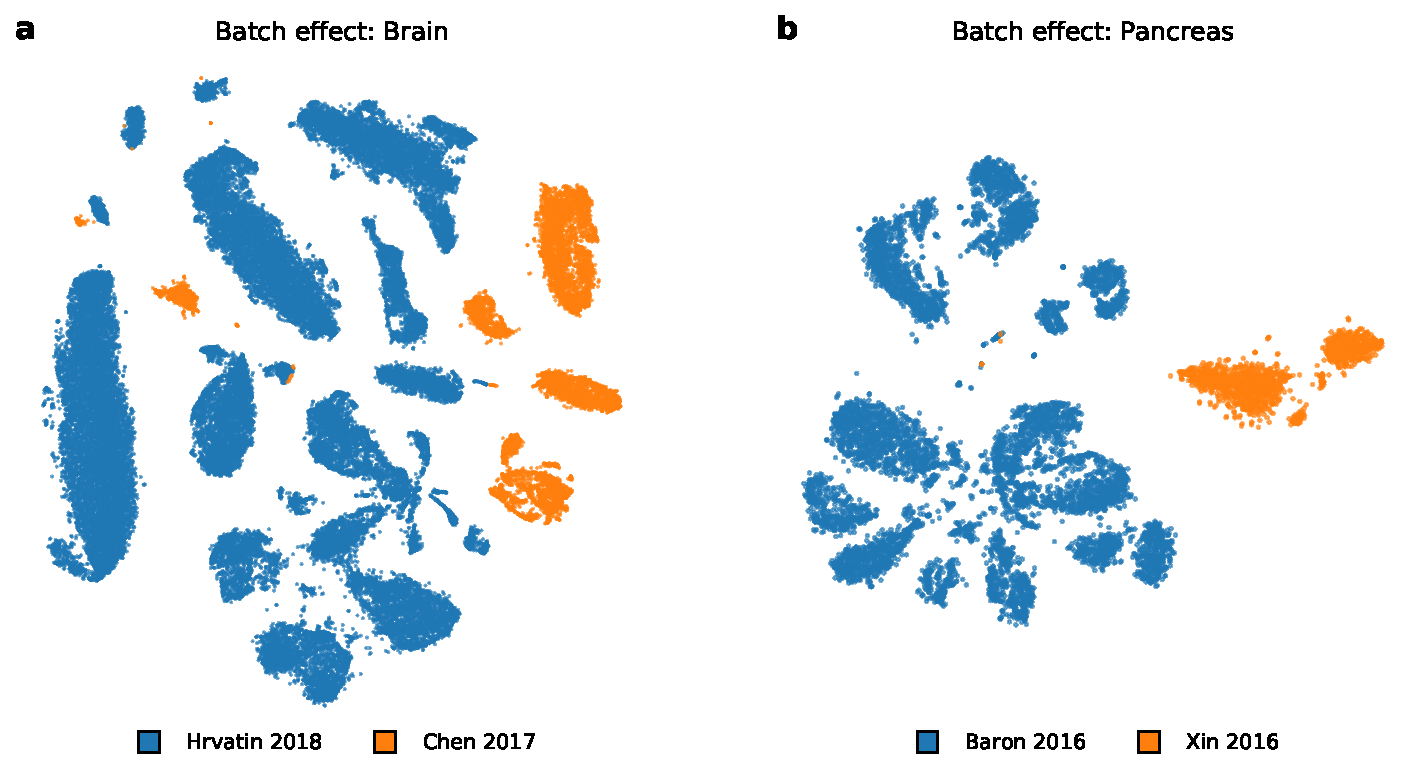
\includegraphics[width=\textwidth]{figures/batch_effect.pdf}
\caption{Batch effects are a driving factor of variation between the data sets.
Depicted is a t-SNE visualisation of two pairs of data sets. In each pair, the
data sets share cell types, so it would be expected that the cells from the
reference data (blue) would mix with the cells in a secondary data sets
(orange). Instead, t-SNE visualisation clusters data according to the data
source.} \label{fig:batch_effect}
\end{figure}

Current solutions to embedding the data from various data sources address the
batch effect problems up-front. The data is typically preprocessed and
transformed such that the batch effects are explicitly
removed. Recently proposed procedures for batch effect removal include
canonical correlation analysis~\cite{cca} and mutual
nearest-neighbors~\cite{mnn,seurat}.
In these works, batch effects are deemed removed when cells from different sources exhibit good mixing in a t-SNE visualization.
The elimination of batch effects may require aggressive data
preprocessing which may blur the boundaries between cell types. Another problem
is also the inclusion of any new data, for which the entire data analysis
pipeline must be rerun, usually resulting in a different layout and clusters
that have little resemblance to original visualization and thus require
reinterpretation.

We propose a direct solution of rendering t-SNE visualizations that addresses
batch effects. Our approach treats one of the data sets as a {\em reference}
and aims to embed the cells from another, {\em secondary data set} to a common low-dimensional space.
We construct a t\nobreakdash -SNE embedding using the reference data set, and then use it
as a scaffold for the embedding of data points from the secondary data.
The key idea underpinning our approach is that the embedding is performed one data point at a time.
Independence of each new
embedded data instance from the secondary data set causes the clustering landscape
to depend only on the reference scaffold, thus removing data source-driven
variation. In other words, when including new data, the scaffold inferred from
the reference data set is kept unchanged and defines a ``gravitational
field'', independently driving the embedding of each new instance. For example, in
Fig.~\ref{fig:transform_brain}, the cells from the visual cortex define the
scaffold (Fig.~\ref{fig:transform_brain}.a) into which we embed the cells from the
hypothalamus (Fig.~\ref{fig:transform_brain}.b). Unlike in their joint t\nobreakdash -SNE
visualization (Fig.~\ref{fig:batch_effect}.a), the hypothalamic cells are
dispersed across the entire embedding space and their cell type correctly matches
the prevailing type in reference clusters.

\begin{figure}[htb]
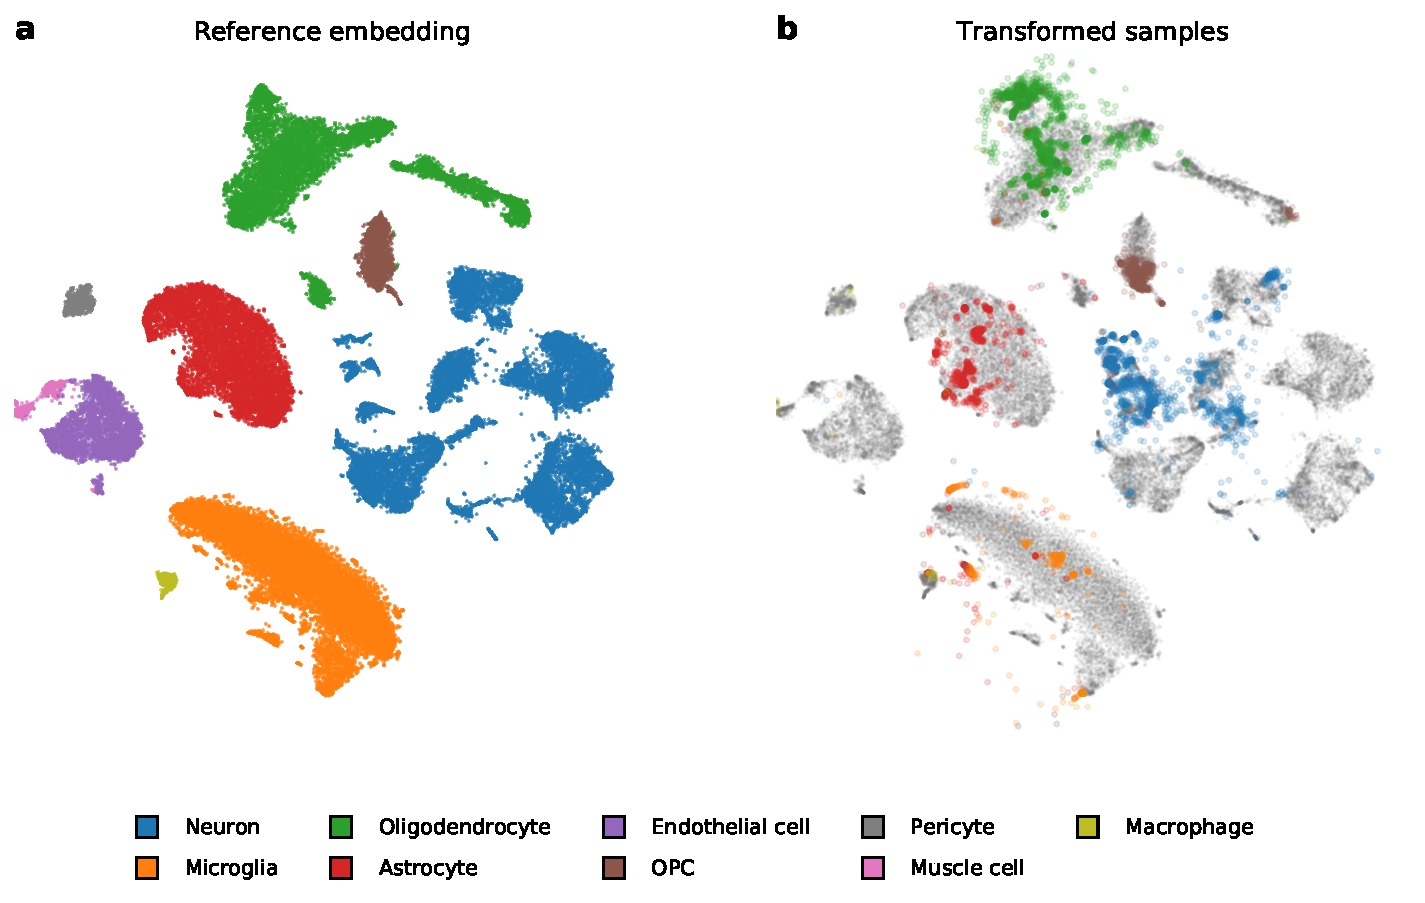
\includegraphics[width=\textwidth]{figures/transform_brain.pdf}
\caption{A two-dimensional embedding of a reference containing brain cells (a) and
the corresponding mapping of secondary data containing hypothalamic cells (b). Notice
that the majority of hypothalamic cells were mapped to their corresponding
reference cluster. For instance, astrocyte cells marked with red on the
right were mapped to an oval cluster of same-typed cells denoted with the same
color in the visualization on the left.} \label{fig:transform_brain}
\end{figure}

The proposed solution is implemented using a mapping of
new data to an existing t-SNE visualization. While the
utility of such an algorithm was already hinted at in recent
publication~\cite{art_of_using_tsne}, here we provide its practical and
theoretically-grounded implementation. Considering the abundance of recent
publications on batch effect removal, we present surprising evidence that a
computationally more direct and principled embedding procedure solves the batch
effects problem when constructing interpretable visualizations from different
data sources.


\section{Methods}

We describe an end-to-end pipeline that uses fixed t-SNE coordinates as a scaffold for
embedding new (secondary) data, enabling joint visualisation of multiple data sources
while mitigating batch effects. Our proposed approach starts by using t\nobreakdash
-SNE to embed a reference data set, with the aim of constructing a
two-dimensional visualisation to facilitate interpretation and cluster
classification. Then, the placement of each new sample is
optimized independently via the
t\nobreakdash -SNE loss function. Independent treatment of each data instance from
a secondary data set disregards any interactions present in that data set, and
prevents the formation of clusters that would be specific to the secondary data. Below, we start
with a summary of t-SNE and its extensions (Sec.~\ref{sec:tsne}, introducing
the relevant notation, upon which we base our secondary data embedding
approach (Sec.~\ref{sec:transfer}).


\subsection{Data embedding by t-SNE and its extensions\label{sec:tsne}}

t-SNE is a local, non-linear dimensionality reduction method, tailored to the visualisation of
high-dimensional data sets. Given a multi-dimensional data set $\mathbf{X} =
\left \{ \mathbf{x}_1, \mathbf{x}_2, \dots, \mathbf{x}_N \right \} \in
\mathbb{R}^D$ where $N$ is the number of samples in the reference data set,
t-SNE aims to find a low dimensional embedding $\mathbf{Y} = \left \{
\mathbf{y}_1, \mathbf{y}_2, \dots, \mathbf{y}_N \right \} \\\in \mathbb{R}^d$
where $d \ll D$, such that if points $\mathbf{x}_i$ and $\mathbf{x}_j$ are
close in the multi-dimensional space, their corresponding embeddings
$\mathbf{y}_i$ and $\mathbf{y}_j$ are also close. Since t-SNE is primarily used
as a visualization tool, $d$ is typically set to two. The similarity between
two data points in t-SNE is defined as:

\begin{equation}
p_{j \mid i} = \frac{\exp \left ( -\frac{1}{2} \mathcal{D}(\mathbf{x}_i, \mathbf{x}_j ) / \sigma_i^2 \right )}
{\sum_{k \neq \i } \exp \left ( -\frac{1}{2} \mathcal{D}(\mathbf{x}_i, \mathbf{x}_k ) / \sigma_i^2 \right )}, \quad p_{i \mid i} = 0
\label{eq:gaussian_kernel}
\end{equation}

\noindent where $\mathcal{D}$ is a distance measure. This is then symmetrized to

\begin{equation}
p_{ij} = \frac{p_{j \mid i} + p_{i \mid j}}{2N}.
\label{eq:symmetrize}
\end{equation}

The bandwidth of each Gaussian kernel $\sigma_i$ is selected such that the
perplexity of the distribution matches a user-specified parameter value

\begin{equation}
\text{Perplexity} = 2^{H(P_i)}
\end{equation}

\noindent where $H(P_i)$ is the Shannon entropy of $P_i$,

\begin{equation}
H(P_i) = -\sum_i p_{j \mid i} \log_2 (p_{j \mid i}).
\end{equation}

\noindent Different bandwidths $\sigma_i$ enable t-SNE to adapt to the varying
density of the data in the multi-dimensional space.

The similarity between points $\mathbf{y}_i$ and $\mathbf{y}_j$ in the
embedding space is defined using the $t$-distribution with one degree of
freedom

\begin{equation}
q_{ij} = \frac{\left ( 1 + || \mathbf{y}_i - \mathbf{y}_j ||^2 \right )^{-1}}
{\sum_{k \neq l}\left ( 1 + || \mathbf{y}_k - \mathbf{y}_l ||^2 \right )^{-1}},
\quad q_{ii} = 0.
\label{eq:cauchy_kernel}
\end{equation}

The t-SNE method finds an embedding $\mathbf{Y}$ that minimizes
the Kullback-Leibler (KL) divergence between $\mathbf{P}$ and $\mathbf{Q}$,

\begin{equation}
C = \text{KL}(\mathbf{P} \mid \mid \mathbf{Q}) = \sum_{ij} p_{ij} \log \frac{p_{ij}}{q_{ij}}.
\label{eq:kl_divergence}
\end{equation}

The time complexity needed to evaluate the similarities in
Eq.~\ref{eq:cauchy_kernel} is $\mathcal{O}(N^2)$, making the application of
the algorithm impractical for any reasonably-sized data. To address larger data
sets, we adopt a recent approach for low-rank approximation of
gradients based on polynomial interpolation which reduces the time
complexity of t-SNE to $\mathcal{O}(N)$. This approximation enables the
visualization of massive data sets, possibly containing millions of data
points~\cite{fi_tsne}.

The resulting embeddings substantially depend on the value of the perplexity
parameter. Perplexity can be interpreted as the number of
neighbors for which the distances in the embedding space are preserved. Small
values of perplexity result in tightly-packed clusters of points and effectively
ignore the long-range interactions between clusters. Larger values may result
in a more globally consistent visualisations, preserving distances on a large
scale and organizing clusters in a more meaningful way. Larger values of
perplexity can lead to merging of multiple small clusters, thus obscuring
local aspects of the data~\cite{art_of_using_tsne}.

The trade-off between the local organization and global consistency may be
achieved by replacing the Gaussian kernels in Eq.~\ref{eq:gaussian_kernel} with
a mixture of Gaussians of varying bandwidths~\cite{multiscale_tsne}.
Multi-scale kernels are defined as

\begin{equation}
p_{j \mid i} \propto \frac{1}{L} \sum_{l=1}^{L} \exp \left ( - \frac{1}{2} \mathcal{D}(\mathbf{x}_i, \mathbf{x}_j ) / \sigma_{i,l}^2 \right ), \quad p_{i \mid i} = 0
\label{eq:multiscale}
\end{equation}

\noindent where $L$ is the number of mixture components. The bandwidths
$\sigma_{i,l}$ are selected in the same manner as in
Eq.~\ref{eq:gaussian_kernel}, but with a different value of perplexity for each
$l$. In our experiments, we used a mixture of two Gaussian kernels with
perplexity values of 50 and 500. We note that a similar formulation of
multi-scale kernels was proposed in~\cite{art_of_using_tsne}, and we found the
resulting embeddings are visually very similar to those obtained with the
approach described above (not shown for brevity).


\subsection{Adding new data points to reference embedding\label{sec:transfer}}

Our algorithm, which embeds new data points to a reference embedding, consists of
estimating similarities between each new point and the reference data and optimizing
the position of each new data point in the embedding space. Unlike parametric models
such as principal component analysis or autoencoders, t-SNE does not define an
explicit mapping to the embedding space, and embeddings need to be found through
loss function optimization.

The position of a new data
point in embedding space is initialized 
to the median reference embedding position of its $k$ nearest 
neighbors. While we found the algorithm to be
robust to choices of $k$, we use $k=10$ in our experiments.

We adapt the standard t-SNE formulation from
Eqs.~\ref{eq:gaussian_kernel}~and~\ref{eq:cauchy_kernel} with

\begin{align}
p_{j \mid i} &= \frac{\exp \left ( -\frac{1}{2} \mathcal{D}(\mathbf{x}_i, \mathbf{v}_j) / \sigma_i^2 \right )}{\sum_{i} \exp \left ( -\frac{1}{2} d(\mathbf{x}_i, \mathbf{v}_j) / \sigma_i^2 \right )}, \\
q_{j \mid i} &= \frac{\left ( 1 + || \mathbf{y}_i - \mathbf{w}_j ||^2 \right )^{-1}}{\sum_{i}\left ( 1 + || \mathbf{y}_i - \mathbf{w}_j ||^2 \right )^{-1}},
\end{align}

\noindent where $\mathbf{V} = \left \{ \mathbf{v}_1, \mathbf{v}_2, \dots,
\mathbf{v}_M \right \} \in \mathbb{R}^D$ where $M$ is the number of samples in
the new data set and $\mathbf{W} = \left \{ \mathbf{w}_1, \mathbf{w}_2, \dots,
\mathbf{w}_M \right \} \in \mathbb{R}^d$. Additionally, we omit the
symmetrization step in Eq.~\ref{eq:symmetrize}. This enables new points to be
inserted into the embedding independently of one another. The gradients of
$\mathbf{w}_j$ with respect to the loss (Eq.~\ref{eq:kl_divergence}) are:

\begin{equation}
\frac{\partial C}{\partial \mathbf{w}_j} = 2 \sum_i \left ( p_{j \mid i} - q_{j \mid i} \right ) \left ( \mathbf{y}_i - \mathbf{w}_j \right ) \left ( 1 + || \mathbf{y}_i - \mathbf{w}_j || ^2 \right )^{-1}
\label{eq:gradient}
\end{equation}

In the optimization step, we refine point positions using batch gradient
descent. We use an adaptive learning rate scheme with momentum 
to speed up the convergence, as proposed by Jacobs~\cite{momentum,bh_tsne}. We run gradient descent
with momentum $\alpha$ set to $0.8$ for $250$ iterations, where the
optimization converged in all our experiments. The time complexity
needed to evaluate the gradients in Eq.~\ref{eq:gradient} is $\mathcal{O}(N
\cdot M)$, however, by adapting the same polynomial interpolation based
approximation, this is reduced to $\mathcal{O}(N)$.

Special care must be taken to reduce the learning rate $\eta$ as the default
value in most implementations ($\eta = 200$) may cause points to ``shoot off''
from the reference embedding. This phenomenon is caused due to the embedding to
a previously defined t-SNE space, where the distances between data points and
corresponding gradients of the optimization function may be quite large. When
running standard t-SNE, points are initialized and scaled to have variance
0.0001. The resulting gradients tend to be very small during the initial phase,
resulting in stable convergence. When embedding new samples, the span of the
embedding is much larger, resulting in substantially larger gradients, and the default
learning rate causes points to move very far from the reference embedding. In
our experiments, we found that decreasing the learning rate to $\eta \sim 0.1$
produces stable solutions. This is especially important when using the
interpolation-based approximation, which places a grid of interpolation
points over the embedding space, where the number of grid points is determined
by the span of the embedding. Clearly, if even one point ``shoots off'' far from the
embedding, the number of required grid points may grow dramatically,
increasing the runtime substantially. The reduced learning rate suppresses this issue, and
does not slow the convergence because of the adaptive learning rate scheme, provided
the optimization is run for a sufficient number of steps. 

\section{Experiments and Discussion}

We apply the proposed approach to t-SNE visualizations of
single-cell data. Data in this realm include a variety of
cells from specific tissues, and characterize them through gene expression.
In our experiments, we considered several recently published data
sets where cells were annotated with the cell type. Our aim was to construct
t-SNE visualizations where similarly-typed cells would cluster together,
despite systematic differences between data sources. Below, we list the data sets,
describe single-cell specific data preprocessing procedures, and display the
resulting data visualizations. Finally, we discuss the success of the proposed
approach in alleviating the batch effects.


\subsection{Data}

We use three pairs of reference and secondary single-cell data sets originating
from different organisms and tissues. The data in each pair were chosen so that
the majority of cell types from the secondary data set were included in the
reference set (Table~\ref{tab:datasets}).

\begin{table}[ht]
\begin{center}
\setlength\tabcolsep{4pt}
\begin{tabular}{l c c r c c}
\toprule
Study & Organism/Tissue & Protocol & Cells & Cell Types & Sparsity (\%) \\
\midrule
Hrvatin \etal & \multirow{2}{*}{mouse brain} & inDrop & 48,266 & 9 & 94 \\
Chen \etal & & Drop-seq & 14,437 & 6 & 93 \\[5pt]
Baron \etal & \multirow{2}{*}{human pancreas} & inDrop & 8,569 & 9 & 91 \\
Xin \etal & & SMARTer & 1,492 & 4 & 86 \\[5pt]
Macosko \etal & \multirow{2}{*}{mouse retina} & Drop-seq & 44,808 & 12 & 97 \\
Shekhar \etal & & Drop-seq & 27,499 & 5 & 96 \\
\bottomrule
\end{tabular}
\end{center}
\caption{Data sets used in our experiments. In each pair, the first data set
(Hrvatin \etal, Baron \etal, and Macoscko \etal) was used as a reference. In
all cases, we relied on the quality control and annotations from the original
publication. To facilitate comparisons, the cell annotations were harmonized using
cell type annotations from the cell ontology~\cite{cell_ontology}. Notice that
different RNA sequencing protocols were used to estimate gene expressions. We
report the number of cell types from each data set retained after
preprocessing. Single-cell data is sparse, typically containing less than 10\%
expressed genes per cell.}
\label{tab:datasets}
\end{table}


The cells in the data sets originates from the following three tissues:
\begin{description}
\item[Mouse brain.] The data set from Hrvatin \etal~\cite{hrvatin2018} contains
cells from the visual cortex exploring transcriptional changes after exposure
to light. This was used as a reference for the data from Chen
\etal~\cite{chen2017}, containing various cells from the mouse hypothalamus and
their reaction to food deprivation. From the secondary data, we removed cells
with no corresponding types in the reference, namely ependymal cells,
epithelial cells, tanycytes, and unlabelled cells.

\item[Human pancreas.] The data set from Baron \etal~\cite{baron2016} was
created as an atlas of pancreatic cell types. We used this set as a reference
for data from Xin \etal~\cite{xin2016}, who examined transcriptional
differences between healthy and type 2 diabetic patients.

\item[Mouse retina.] The data set from Macosko \etal~\cite{macosko2015} was
created as an atlas of mouse retinal cell types. We used this as a reference
for the data from Shekhar \etal~\cite{shekhar2016}, who built an atlas for
different types of retinal bipolar cells.
\end{description}

\subsection{Single-cell data preprocessing pipeline}

Due to the specific nature of single-cell data, additional steps must be taken
to properly apply t-SNE. We use a standard single-cell preprocessing pipeline,
consisting of the selection of 3,000 representative genes (see
Sec.~\ref{sec:gene-selection}), library size normalization, log-transformation,
standardization, and PCA-based representation that retains 50 principal
components~\cite{seurat,scanpy}. To obtain the reference embedding, we apply
multi-scale t-SNE using PCA initialization~\cite{art_of_using_tsne}. Due to
high-dimensionality of the preprocessed input data we use cosine distance to
estimate similarities between reference data points~\cite{Domingos2012-CACM}.
When adding new data points from the secondary data set to the reference embedding,
we select 1,000 genes present in both data sets and use these to estimate the
similarities between the secondary data item and reference data points. The
similarities are estimated using cosine similarity. We note that similarities are
computed using the raw count matrices. The preprocessing stages are detailed in
accompanying Python notebooks (Sec.~\ref{sec:implementation}).

\subsection{Gene selection\label{sec:gene-selection}}

Single-cell data sets suffer from high levels of technical noise and low
capture efficiency, resulting in sparse expression matrices~\cite{umi}. To
address this problem, we use a specialized feature-selection method, which
exploits the mean-dropout relationship of expression counts as recently
proposed by Kobak and Berens~\cite{art_of_using_tsne}. Here, genes with higher
than expected dropout rate are regarded as potential markers for cell
subpopulations and are retained in the data.

Given an expression matrix $\mathbf{X} \in \mathbb{R}^{N \times G}$ where $N$
is the number of samples and $G$ is the number of genes in the data set, we
compute the fraction of cells where a gene $g$ was not expressed

\begin{equation}
d_g = \frac{1}{N} \sum_i I \left ( X_{ig} = 0\right )
\end{equation}

\noindent The mean $\log_2$ expression of the genes is computed from all the
cells where gene was expressed:

\begin{equation}
m_g = \left \langle \, \log_2 X_{ig} \mid X_{ig} > 0 \, \right \rangle.
\end{equation}

All genes expressed in less than ten cells are discarded. In order to select a
specific number of $\hat{G}$ genes, we use a binary search to find a value $b$
such that

\begin{equation}
\sum_g I \left (d_g > \exp \left [ -(m_g - b) \right ] + 0.02 \right ) = \hat{G}.
\end{equation}

\subsection{Results and Discussion}

Figs.~\ref{fig:transform_brain}, \ref{fig:transform_pancreas}, and
\ref{fig:transform_retina} show the embeddings of the reference data sets and
their corresponding embeddings of the secondary data sets. In all the figures,
the cells from the secondary data sets were positioned in the cluster of
same-typed reference cells, providing strong evidence of the success of the
proposed approach. There are some deviations to these observations; for
instance, in Fig.~\ref{fig:transform_brain} several oligodendrocyte precursor
cells (OPCs) were mapped to oligodendrocytes. This may be due to differences in
annotation criteria by different authors, or due to inherent similarities of
these types of cells. Examples of such erroneous placements can be found in
other figures as well, but they are not common and constitute less then 5\% of
the cells (less than  5\% in brain, \%1 in pancreas and \%2 in retina
secondary data sets).

Notice that we could simulate the split between reference and secondary data
sets using one data set only and perform cross-validation, however this type of experiment
would not incorporate batch effects. We want to remind the reader that handling
batch effects were central to our endeavour and that the disregard of this effect
could lead to overly-optimistic results and data visualizations strikingly different from ours. For example,
compare the visualisations from Fig.~\ref{fig:batch_effect}.a and
Fig.~\ref{fig:transform_brain}.b, or Figs.~\ref{fig:batch_effect}.b and
\ref{fig:transform_pancreas}.b.

\begin{figure}[htb]
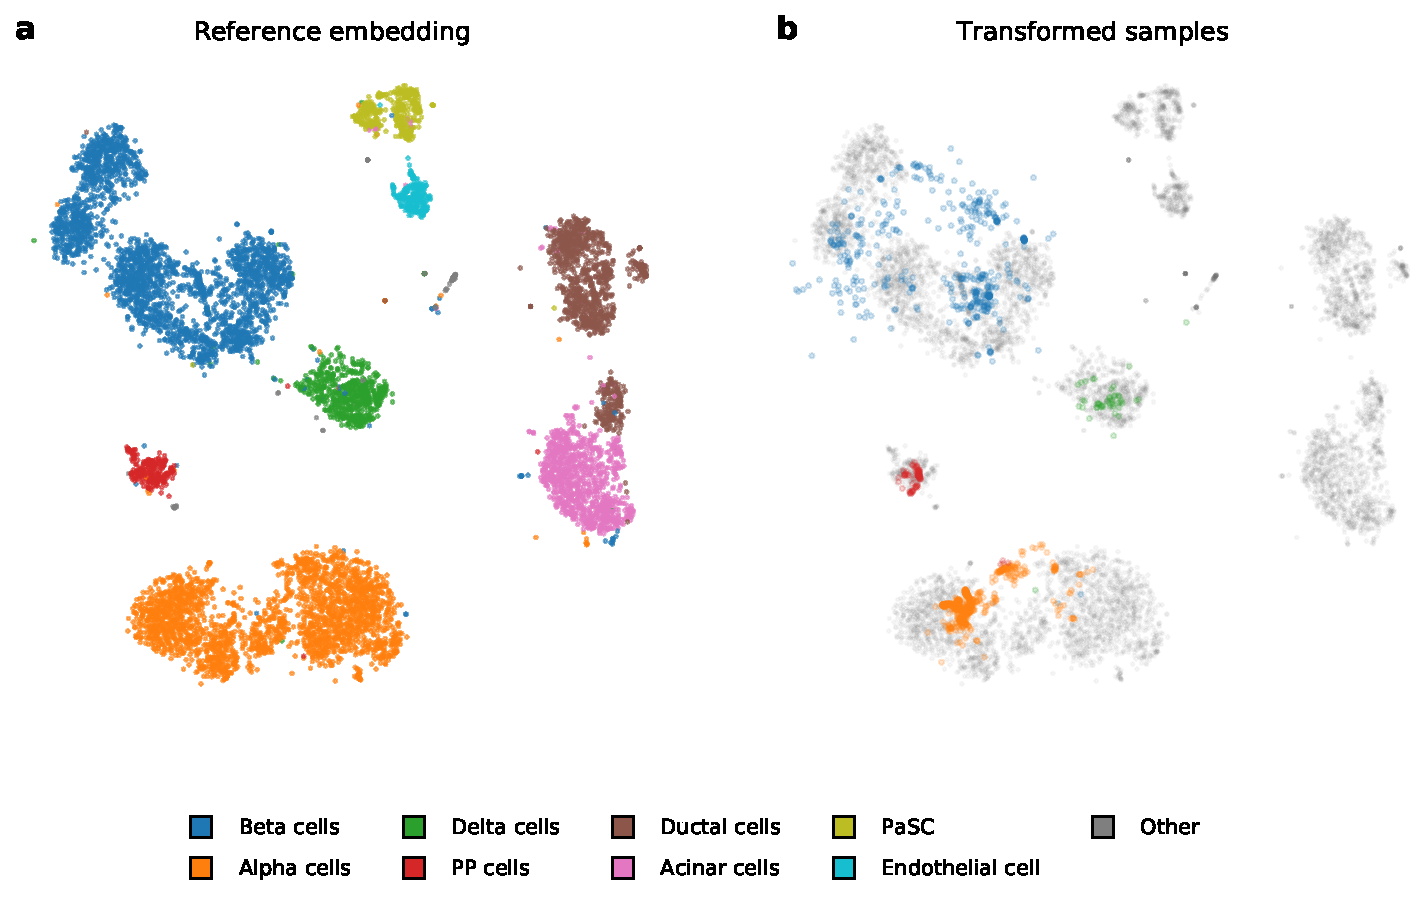
\includegraphics[width=\textwidth]{figures/transform_pancreas.pdf}
\caption{Embedding of pancreatic cells from Baron \etal~\cite{baron2016} and
cells from the same tissue from Xin \etal.~\cite{xin2016}. Just like in
Fig.~\ref{fig:transform_brain} the vast majority of the cells from the secondary
data set were correctly mapped to the same-typed cluster of reference
cells.}\label{fig:transform_pancreas}
\end{figure}


\begin{figure}[htb]
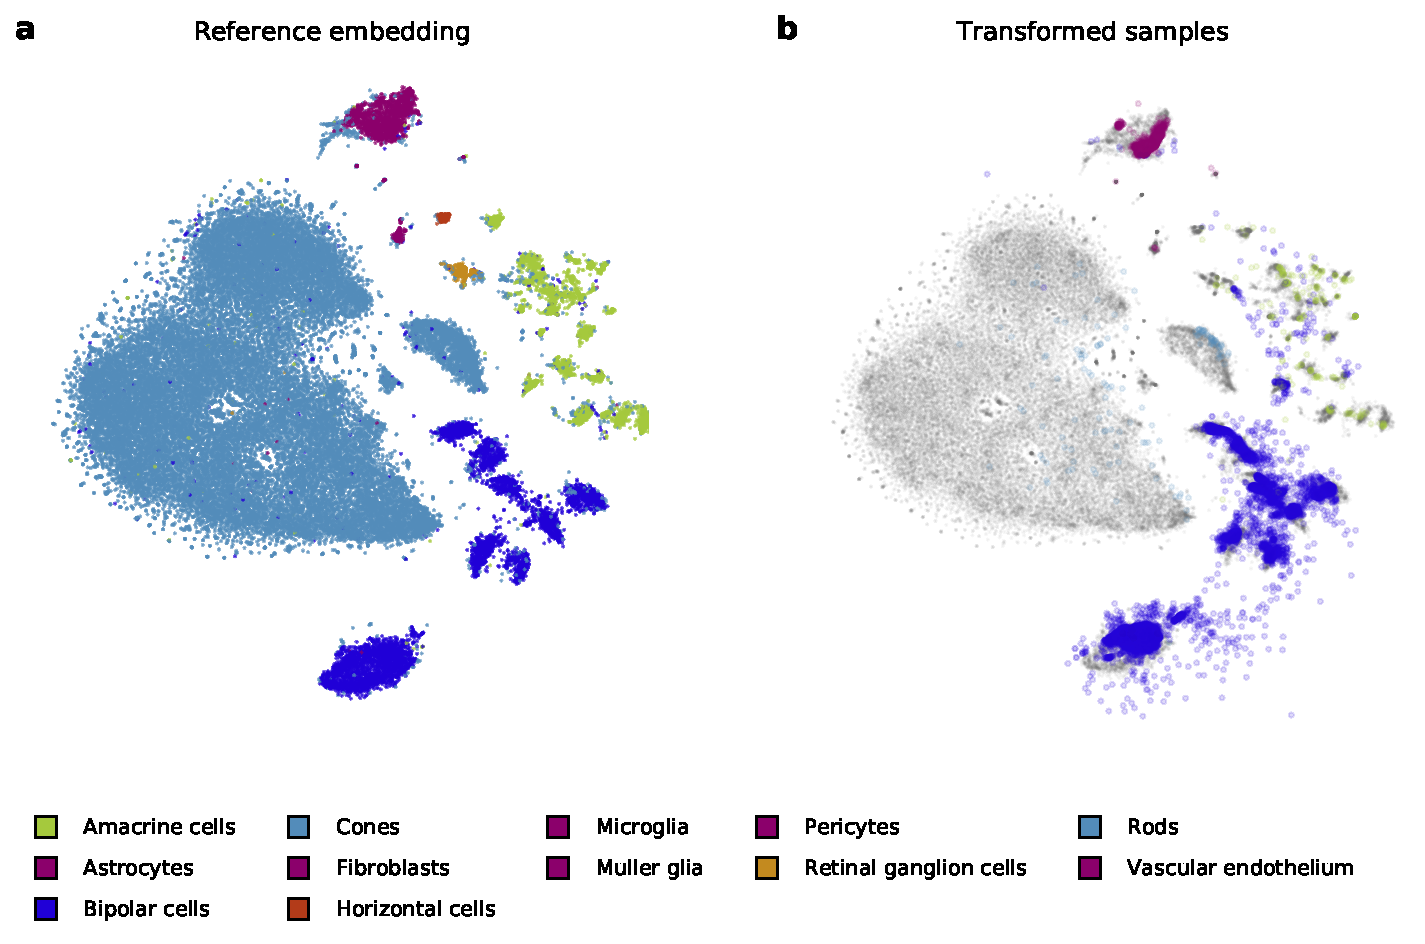
\includegraphics[width=\textwidth]{figures/transform_retina.pdf}
\caption{An embedding of a large reference of retinal cells from Macosco
\etal~\cite{macosko2015} (a) and mapping of cells from a smaller study that
focuses on bipolar cells from Shekhar \etal~\cite{shekhar2016} (b). We use
colors consistent with the study by Macosko \etal.} \label{fig:transform_retina}
\end{figure}

There are additional modifications that we use in the embedding of the
secondary data set that were recently proposed and enhance the original t-SNE visualization.
One important extension is the use of multi-scale similarities that, besides local ordering of the
data points, includes global optimization of cluster placement. For
illustration, consider visualizations with standard and multi-scale t-SNE in
Fig.~\ref{fig:multiscale}. Notice, for instance, that in multi-scale t-SNE
(Fig.~\ref{fig:multiscale}.b) the clusters with neuronal cells are clumped
together, while their placement in standard t-SNE is arbitrary
(Fig.~\ref{fig:multiscale}.a).


\begin{figure}[htbp]
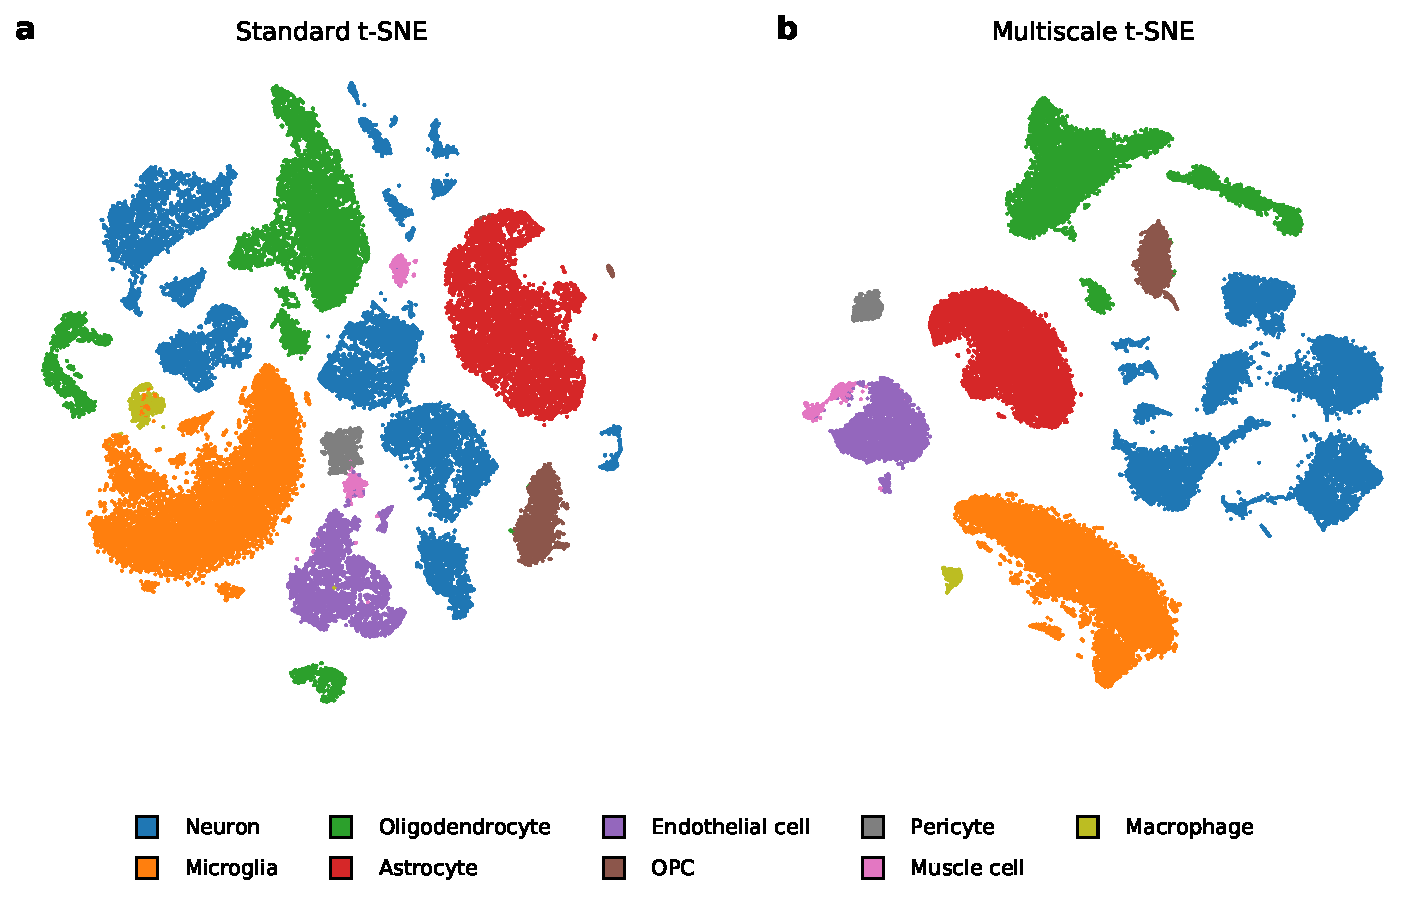
\includegraphics[width=\textwidth]{figures/hrvatin_multiscale_tsne.pdf}
\caption{A comparison of standard and multi-scale t-SNE on data
from the mouse visual cortex~\cite{hrvatin2018}. {\bf (a)} Standard t-SNE
places clusters arbitrarily. {\bf (b)} Augmenting t-SNE with multi-scale
similarities and using proper initialization provides a more meaningful layout of the clusters. Neuronal types
occupy one region of the space. Oligodendrocyte precursor cells (OPCs) are
mainly progenitors to oligodendrocytes, but may also differentiate into neurons
or astrocytes.} \label{fig:multiscale}
\end{figure}

We also observed the important role of gene selection in crafting the
reference embedding spaces. We found that when selecting an insufficient
number of genes, the resulting visualizations display overly-fragmented clusters. When
the selection is too broad and includes lowly expressed genes, the subclusters
tend to overlap. These effects can all be attributed to sparseness of the data
sets and may be intrinsic to single-cell data. In our studies, we found that
selection of 3,000 genes yields most informative visualizations
(Fig.~\ref{fig:gene_selection}).

\begin{figure}[htbp]
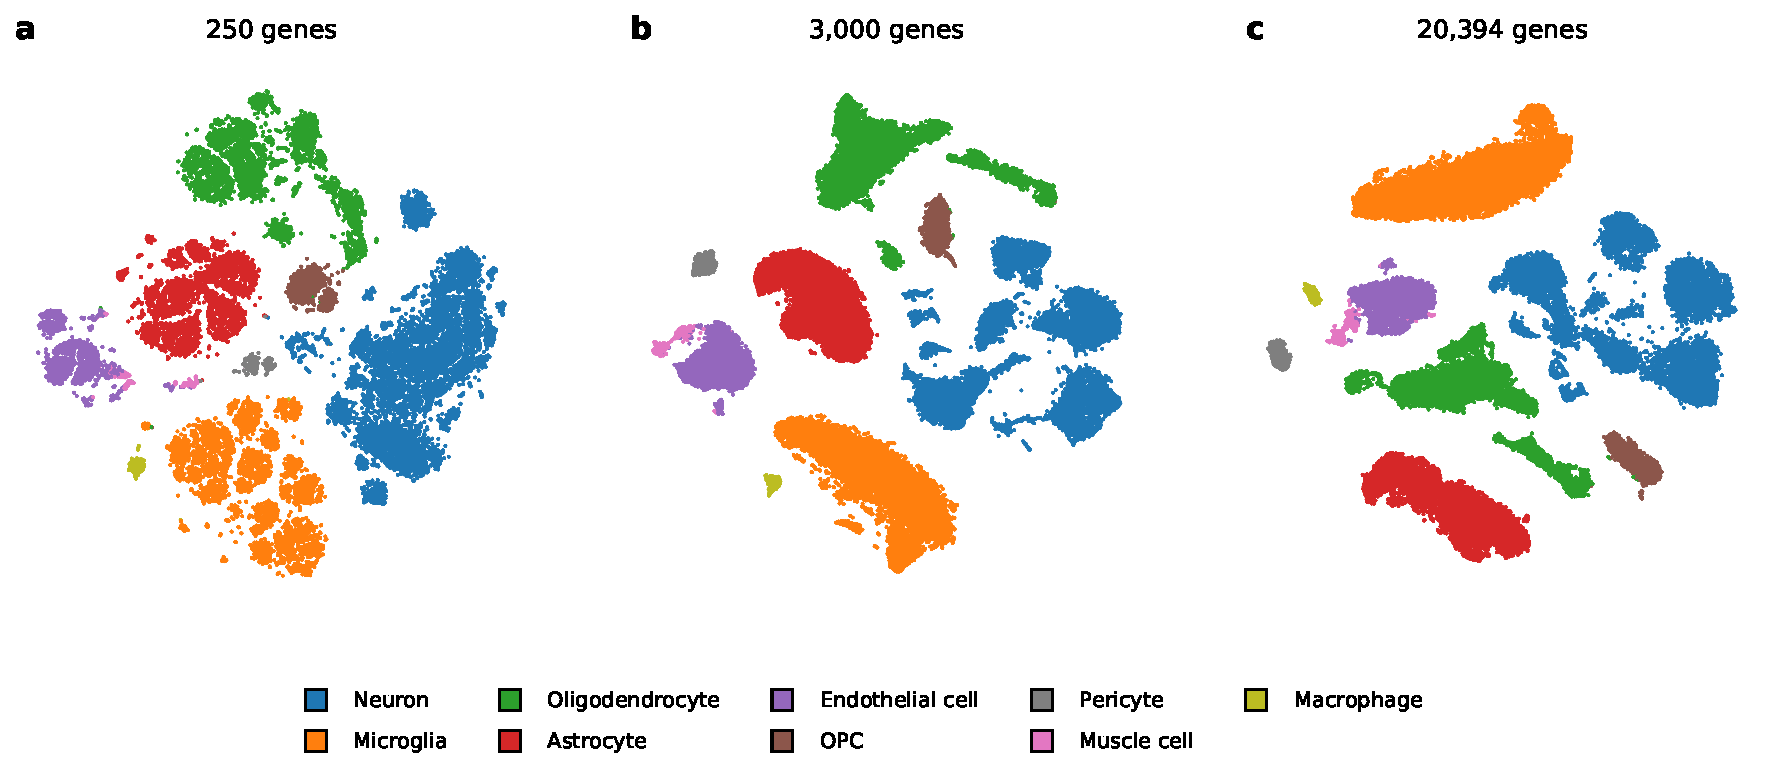
\includegraphics[width=\textwidth]{figures/hrvatin_embedding_tsne_genes.pdf}
\caption{Gene selection plays an important role when constructing the reference
embedding. {\bf (a)} Using too few genes results in fragmented clusters. {\bf (b)}
Using an intermediate number of genes reveals clustering mostly consistent with
cell annotations. {\bf (c)} Including all the genes may lead to
under-clustering of the more specialized cell types.}
\label{fig:gene_selection}
\end{figure}

In principle, our theoretically-grounded embedding of secondary data into the
scaffold defined by the reference embedding could be simplified with the
application of the nearest neighbors-based procedure. For example, while
describing a set of tricks for t-SNE, Kobak and Berens~\cite{art_of_using_tsne}
proposed positioning new points into a known embedding by placing them in the
median position of their 10 nearest neighbors, where the neighborhood was
estimated in the original data space. Notice that we use this approach as well,
but only for the initialization of positions of new data instances that are subject
to further optimization. In Fig.~\ref{fig:optimization} we demonstrate that
nearest neighbor-based positioning is insufficient and may yield clumped
visualizations where the optimal positioning using the t-SNE loss function is
much more dispersed and rightfully shows a more considerable variation in the
secondary data. Some data points may also fall into the empty regions
between different clusters, while after optimization they typically
move closer to same-typed groups.

\begin{figure}[htbp]
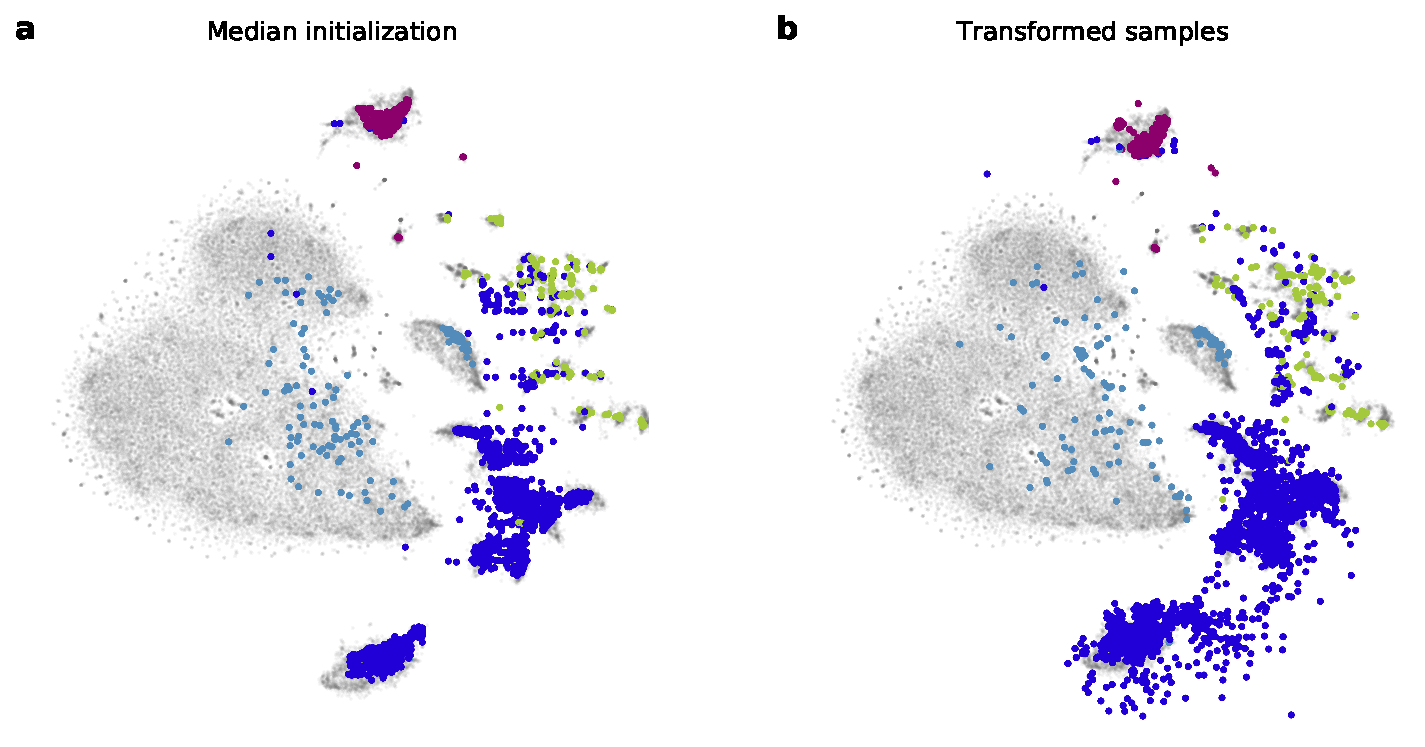
\includegraphics[width=\textwidth]{figures/optimization_retina.pdf}
\caption{Comparison of data placement using the nearest neighbors approach from Kobak
and Berens~\cite{art_of_using_tsne} and the optimized placement using our algorithm.
{\bf (a)} Data points are placed to the median position of their 10 nearest
neighbors in the reference set. {\bf (b)} Point positions are optimized,
revealing a different, more dispersed placement that better reflects the
variety of cells in the secondary data set.}
\label{fig:optimization}
\end{figure}

The proposed method assumes that all cell types from the secondary data set are
present in the reference. The proposed method would fail to reveal novel cell
types in the secondary data set, possibly positioning them arbitrarily close to
unrelated clusters. Procedures such as scmap were recently
proposed to cope with such cases and identify the cells whose type is new and
not included in the reference~\cite{scmap}. Our procedure does not address such cases, and
for scaling-up to a wider collection of cell types relies on emerging
availability of large collections of the reference data such as those managed
by Human Cell Atlas initiative~\cite{hca}. 

\subsection{Implementation\label{sec:implementation}}

The procedures described in this paper are provided as Python notebooks that
are, together with the data, available in an open
repository~\footnote{https://github.com/biolab/tsne-embedding}. All experiments
were run using openTSNE~\footnote{https://github.com/pavlin-policar/openTSNE},
our open and extensible t-SNE library for Python.

\section{Conclusion}

Almost all recent publications of single-cell studies begin with a
two-dimensional visualization of the data that reveals the cellular diversity containing many 
different cell-types from the study. While any dimensionality reduction
technique can be used to render such a visualization, different variants of
t-SNE are most often used. Due to the ability to explore biological mechanisms
at the individual cell level, single-cell studies are increasingly widespread, and
their publications in the past couple of years are abundant. One of the central
tasks in single-cell studies is the classification of new cells based on
findings from previous studies. Such transfer of knowledge is often difficult
due to batch effects present in data from different sources.
Addressing batch effects by adapting and extending t-SNE, the prevailing method used
to present single-cell data in two-dimensional visualization motivated the research
presented in this paper. 

Our proposed approach uses a t-SNE embedding as a scaffold for the positioning of
new cells within the visualization, and possibly for aiding in their
classification. The three case studies incorporating pairs of data sets from
different domains but with similar classifications demonstrate that our
proposed procedure can effectively deal with batch effects to construct
visualizations that correctly map secondary data sets onto a reference data
set from an independent study that possibly uses different experimental
protocol. While we focused here on reference visualizations constructed using t-SNE,
this approach can be applied using any existing two-dimensional visualization.

\subsubsection*{Acknowledgements}

This work was supported by the Slovenian Research Agency Program Grant P2-0209,
and by the BioPharm.SI project supported from European Regional Development
Fund and the Slovenian Ministry of Education, Science and Sport. We would also
like to thank Dmitry Kobak for discussions on t-SNE.

% \bibliographystyle{splncs04}
\bibliographystyle{unsrt}
\bibliography{references}
\end{document}
